\documentclass[compress]{beamer}
\usepackage{ifthen,verbatim}

\title{Pre-CSA07 Exercises: \\ Validation of 1\_5\_4 Samples}
\author{Jim Pivarski, Alexei Safonov}
\institute{Texas A\&M University}
\date{27 August, 2007}

\newcommand{\isnote}{}
\xdefinecolor{lightyellow}{rgb}{1.,1.,0.25}
\xdefinecolor{darkblue}{rgb}{0.1,0.1,0.7}

%% Uncomment this to get annotations
%% \def\notes{\addtocounter{page}{-1}
%%            \renewcommand{\isnote}{*}
%% 	   \beamertemplateshadingbackground{lightyellow}{white}
%%            \begin{frame}
%%            \frametitle{Notes for the previous page (page \insertpagenumber)}
%%            \itemize}
%% \def\endnotes{\enditemize
%% 	      \end{frame}
%%               \beamertemplateshadingbackground{white}{white}
%%               \renewcommand{\isnote}{}}

%% Uncomment this to not get annotations
\def\notes{\comment}
\def\endnotes{\endcomment}

\setbeamertemplate{navigation symbols}{}
\setbeamertemplate{headline}{\includegraphics[height=1 cm]{../cmslogo} \hspace{0.1 cm} \includegraphics[height=1 cm]{../tamulogo} \hfill
\begin{minipage}{5.5 cm}
\vspace{-0.75 cm} \small
\begin{center}
\ifthenelse{\equal{\insertpagenumber}{1}}{}{\textcolor{blue}{\insertsection}}
\end{center}
\end{minipage} \hfill
\begin{minipage}{4.5 cm}
\vspace{-0.75 cm} \small
\begin{flushright}
\ifthenelse{\equal{\insertpagenumber}{1}}{}{Jim Pivarski \hspace{0.5 cm} \insertpagenumber\isnote/\pageref{numpages}}
\end{flushright}
\end{minipage}\mbox{\hspace{0.2 cm}}}

\begin{document}
\frame{\titlepage}

\begin{notes}
\item This is the annotated version of my talk.
\item If you want the version that I am presenting, download the one
labeled ``slides'' on Indico (or just ignore these yellow pages).
\item The annotated version is provided for extra detail and a written
record of comments that I intend to make orally.
\item Yellow notes refer to the content on the {\it previous} page.
\item All other slides are identical for the two versions.
\end{notes}

\begin{frame}
\frametitle{Last Friday's AlCa meeting}
\begin{itemize}\setlength{\itemsep}{0.3 cm}
\item I had some I/O troubles filtering 1\_5\_4 $Z\to\mu\mu$ samples for alignment tests (``converting to AlCaReco format'')
\item This will be produced officially sometime this week: I'll wait for that
\item I did get to look at 10,000 ideal and short-term misalignment/miscalibration events
\item (AlCa group will also produce miscalibrated but not misaligned samples)
\item The following plots confirm that the ideal and short-term are
what they claim to be, and I'll be able to do systematics studies with
the 1\_5\_4 samples
\end{itemize}
\end{frame}

\begin{frame}
\frametitle{Z peak in short-term scenario}

globalMuons, refit to tracker-only

\begin{center}
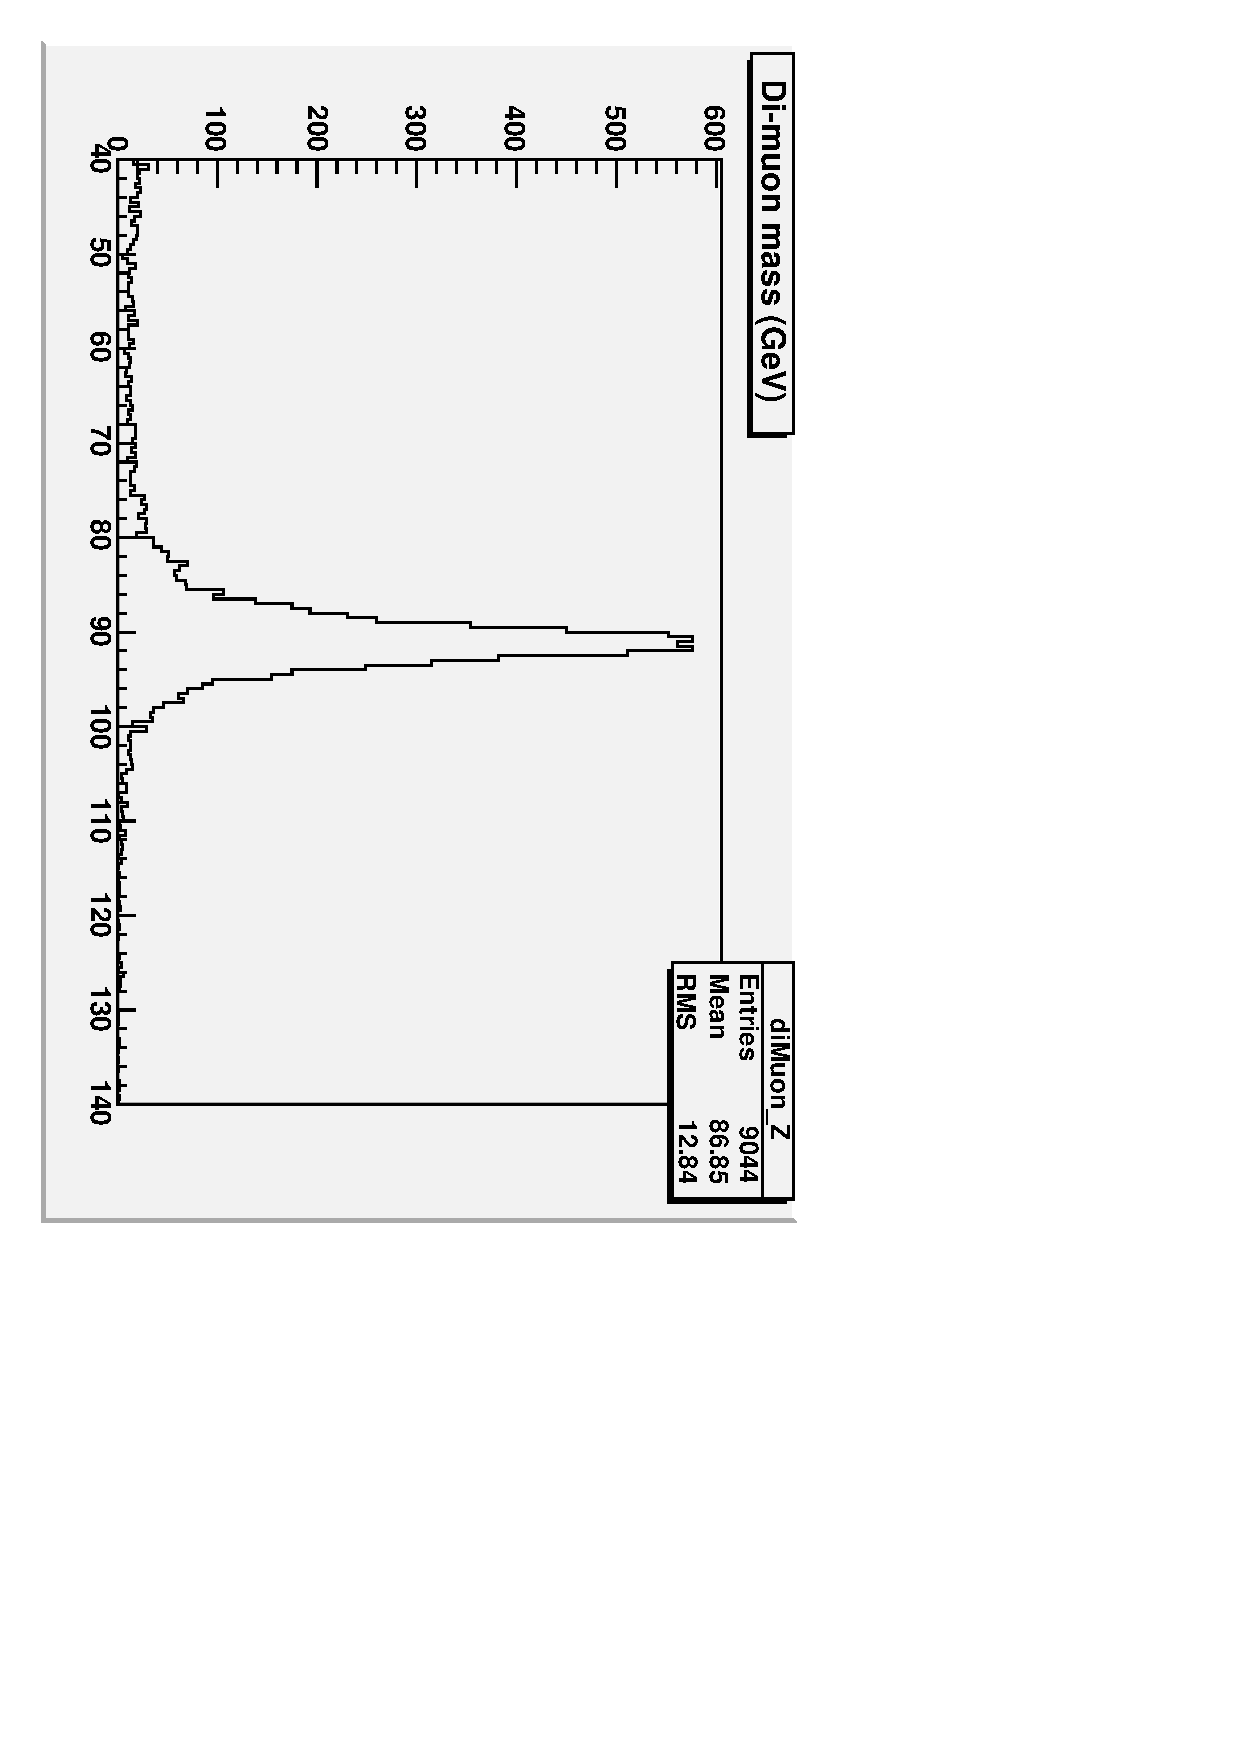
\includegraphics[height=0.7\linewidth, angle=90]{deweighted_short_zpeak.pdf}
\end{center}

Confirms that event generation is okay and tracker is okay: says
nothing about muon system
\end{frame}

\begin{frame}
\frametitle{Residuals in the muon system}

\begin{itemize}
\item Again, tracks fitted to the tracker, projected into the muon system
\end{itemize}

\begin{center}
\begin{tabular}{p{0.45\linewidth} p{0.45\linewidth}}
\begin{minipage}{\linewidth}
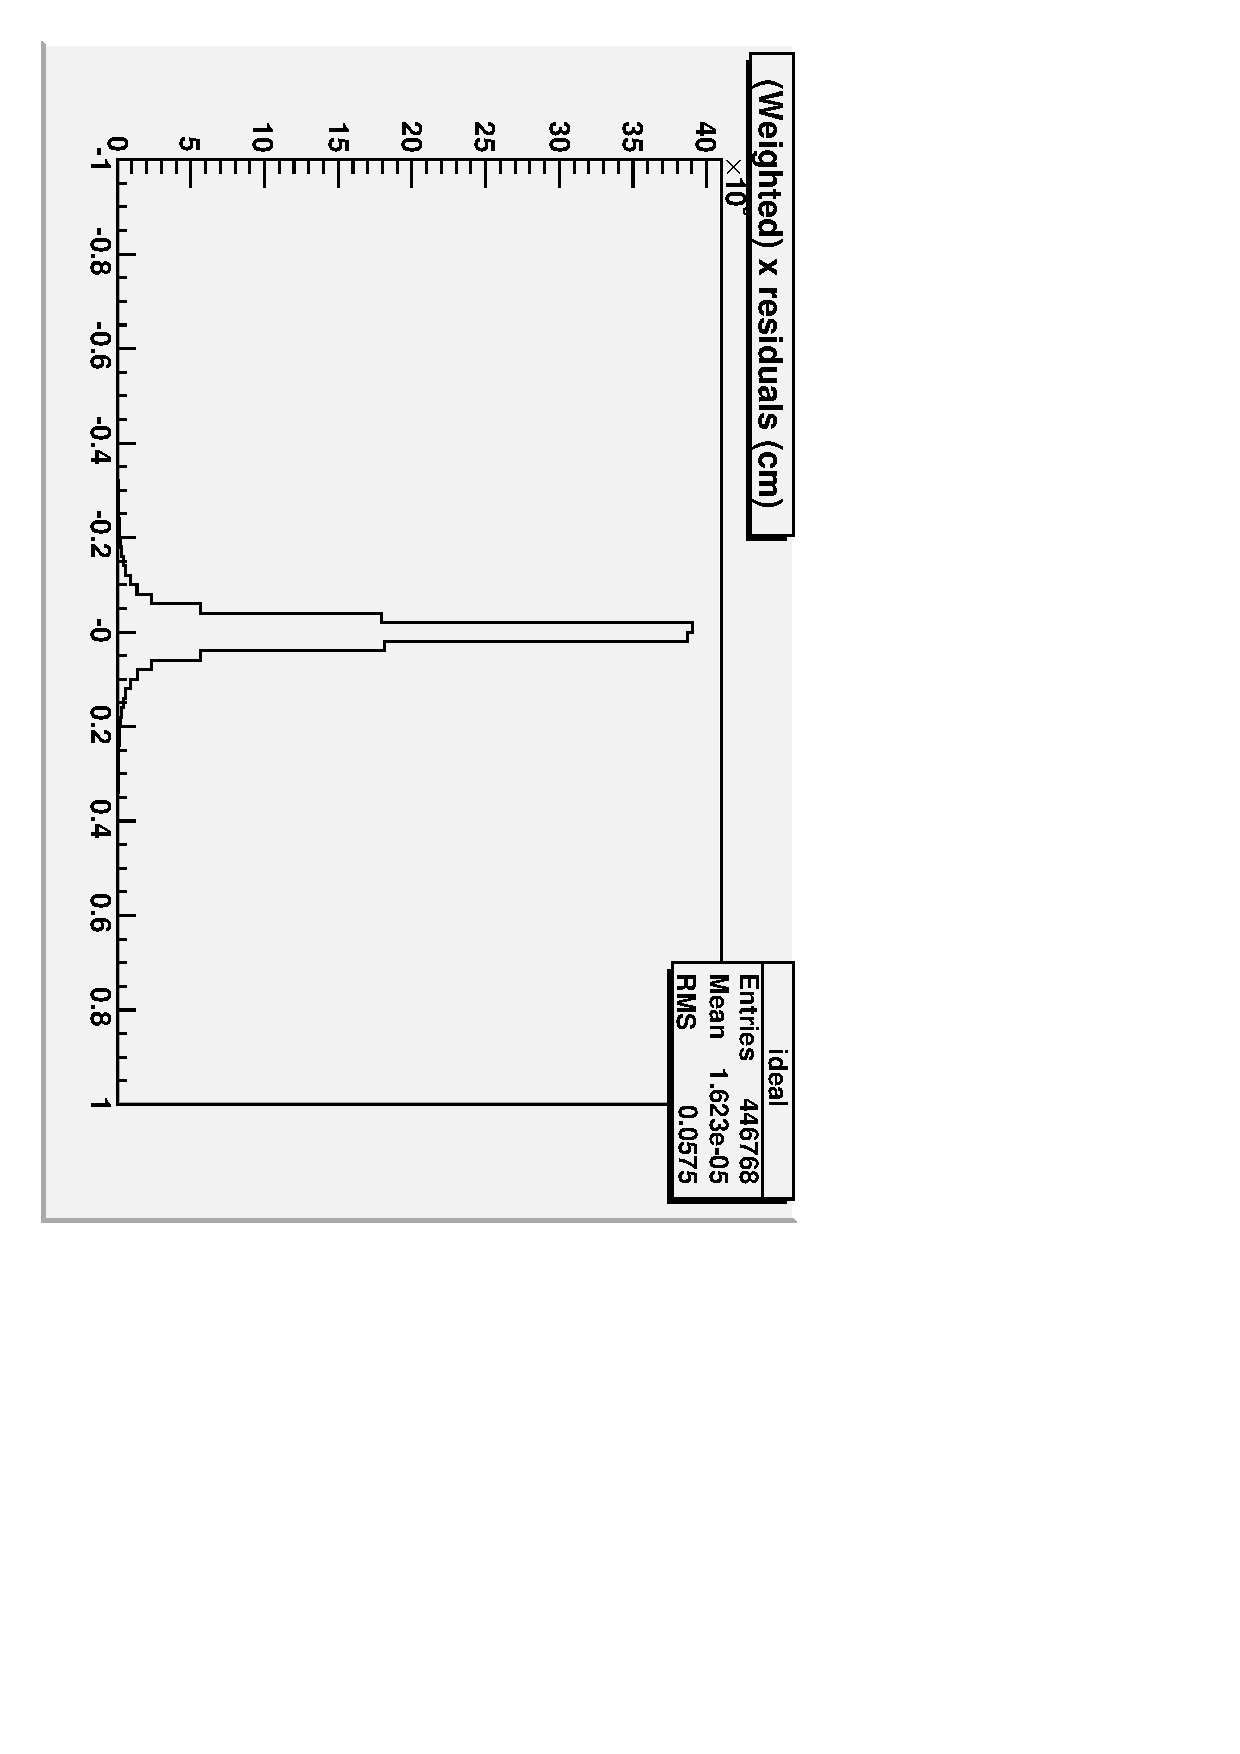
\includegraphics[height=\linewidth, angle=90]{deweight_outin_ideal.pdf}
\end{minipage} &
\begin{minipage}{\linewidth}
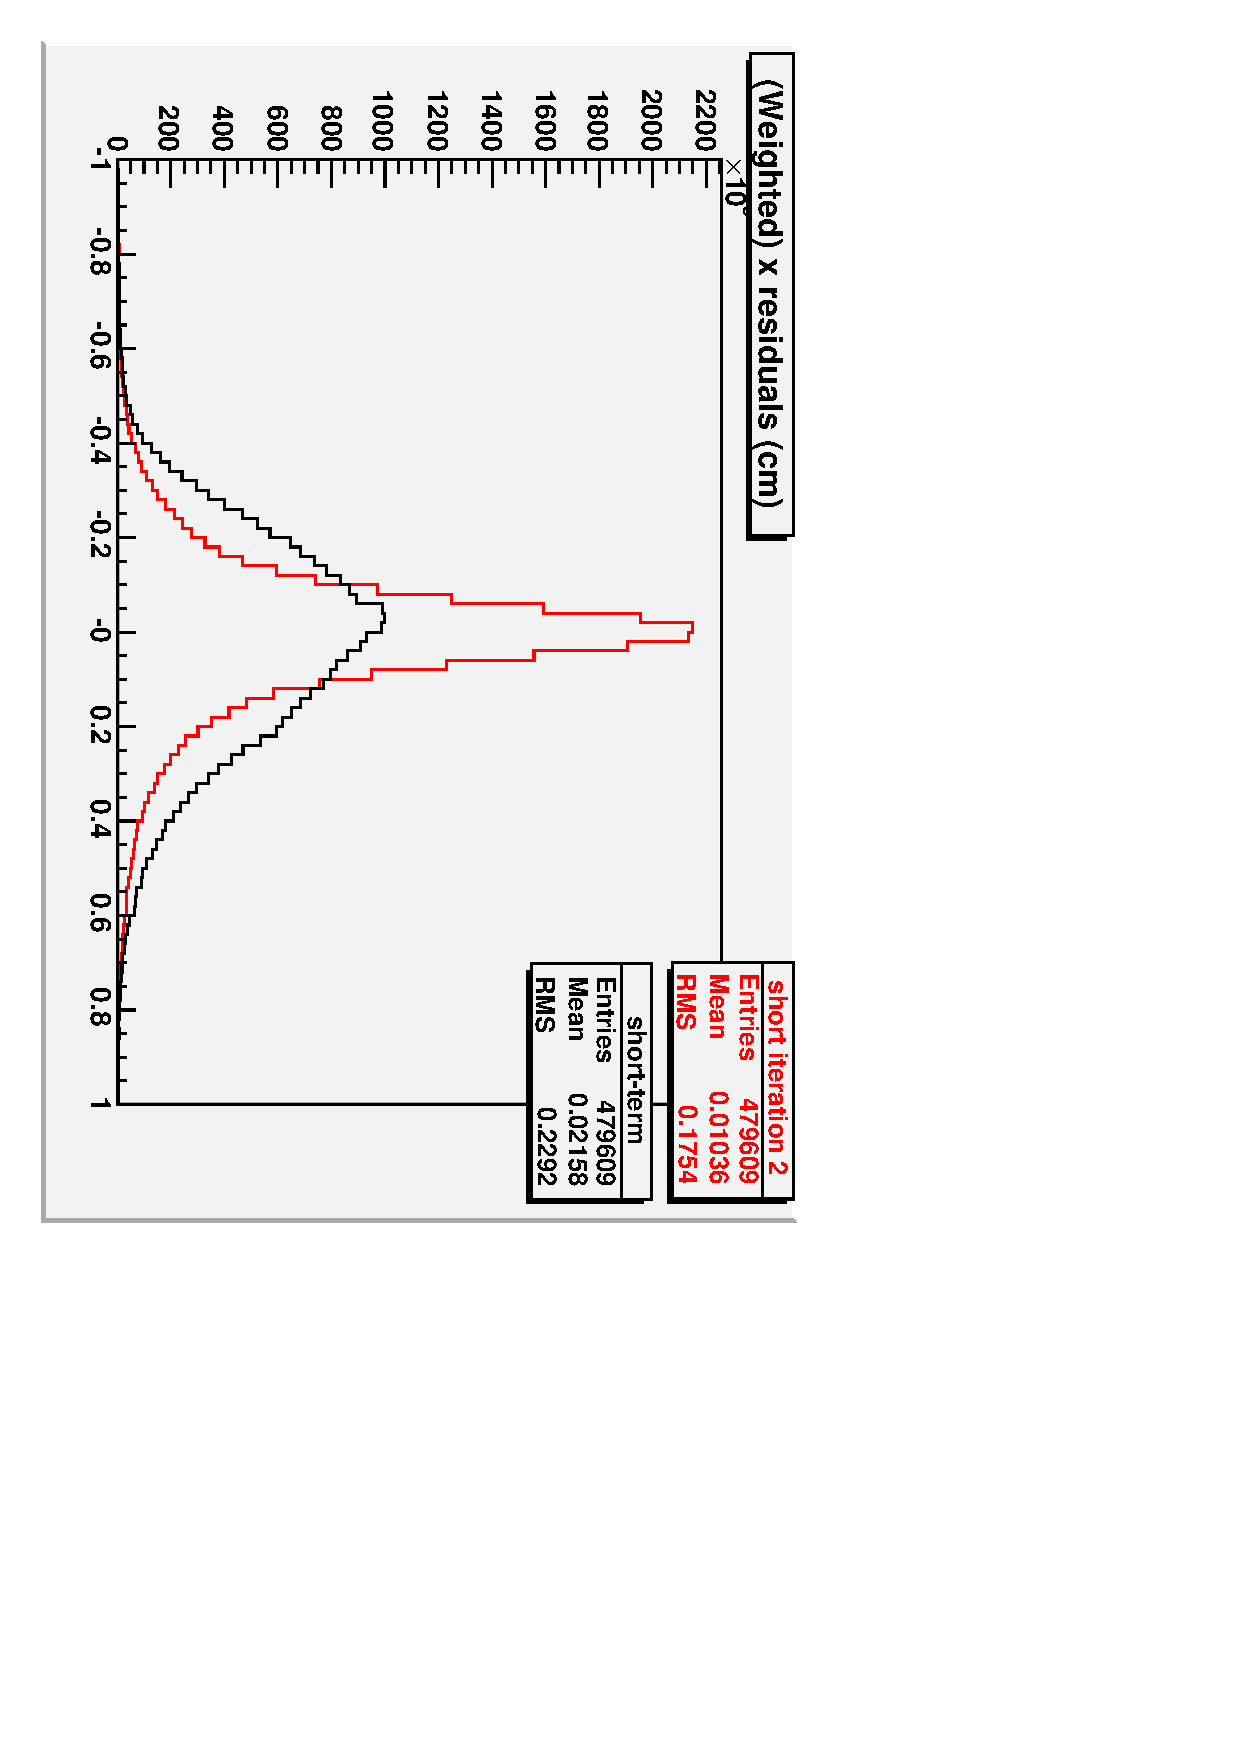
\includegraphics[height=\linewidth, angle=90]{deweight_outin_short.pdf}
\end{minipage} \\
\begin{minipage}{\linewidth}
\begin{center}
Ideal align/calib
\end{center}
\end{minipage} &
\begin{minipage}{\linewidth}
\begin{center}
Short-term scenario (10 pb$^{-1}$)
\end{center}
\end{minipage}
\end{tabular}
\end{center}

\vfill \textcolor{red}{Red} short-term is a quickie alignment: $x$ and
$\phi_z$ only, chamber-by-chamber, one iteration ($\sim$300/790 chambers aligned).

\vfill RMS from 2.3 mm $\to$ 1.8 mm, with ideal being 0.6 mm
\end{frame}

%% \begin{frame}
%% \frametitle{Typical single-chamber residuals distribution \#1}
%% \begin{center}
%% 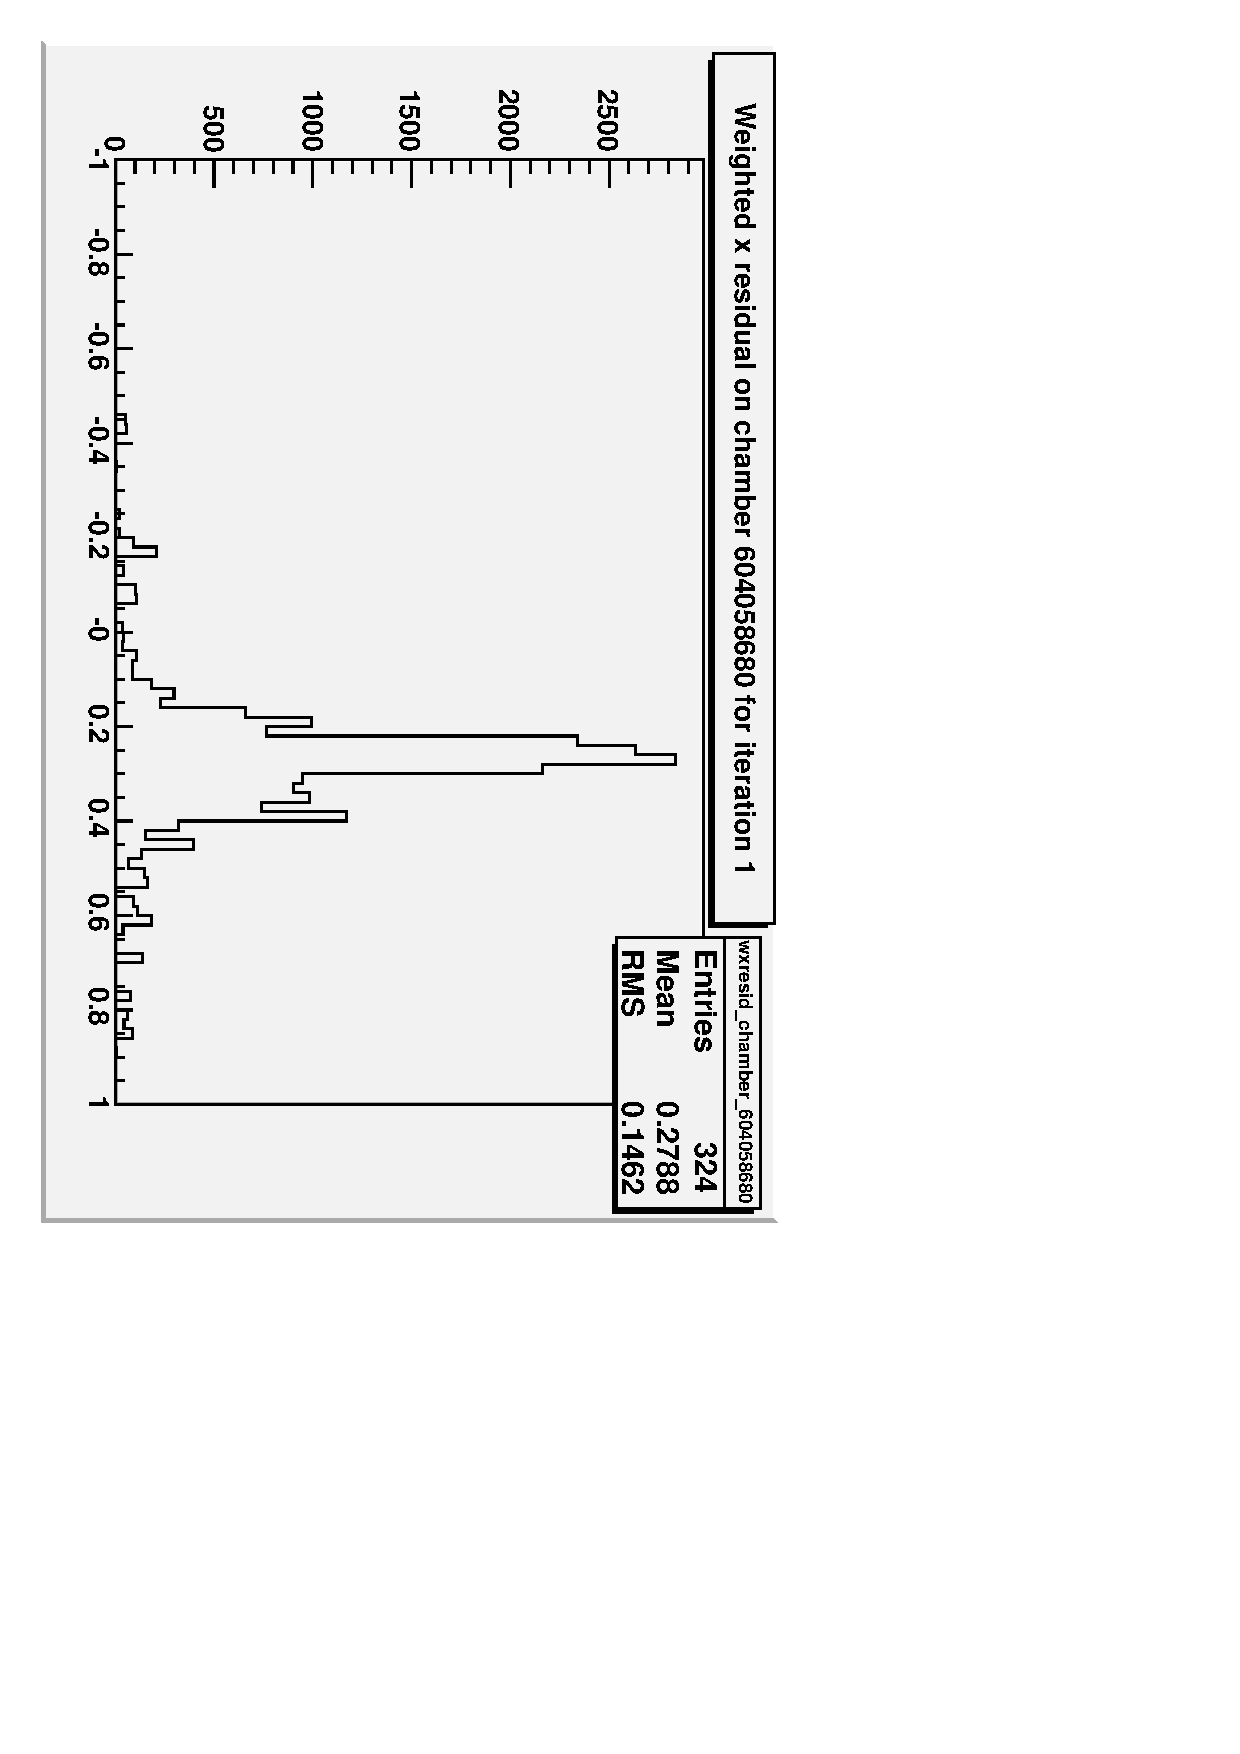
\includegraphics[height=0.7\linewidth, angle=90]{typical_short_deweight_outin.pdf}
%% \end{center}

%% \vfill
%% Cleanly misaligned
%% \end{frame}

%% \begin{frame}
%% \frametitle{Typical single-chamber residuals distribution \#2}
%% \begin{center}
%% 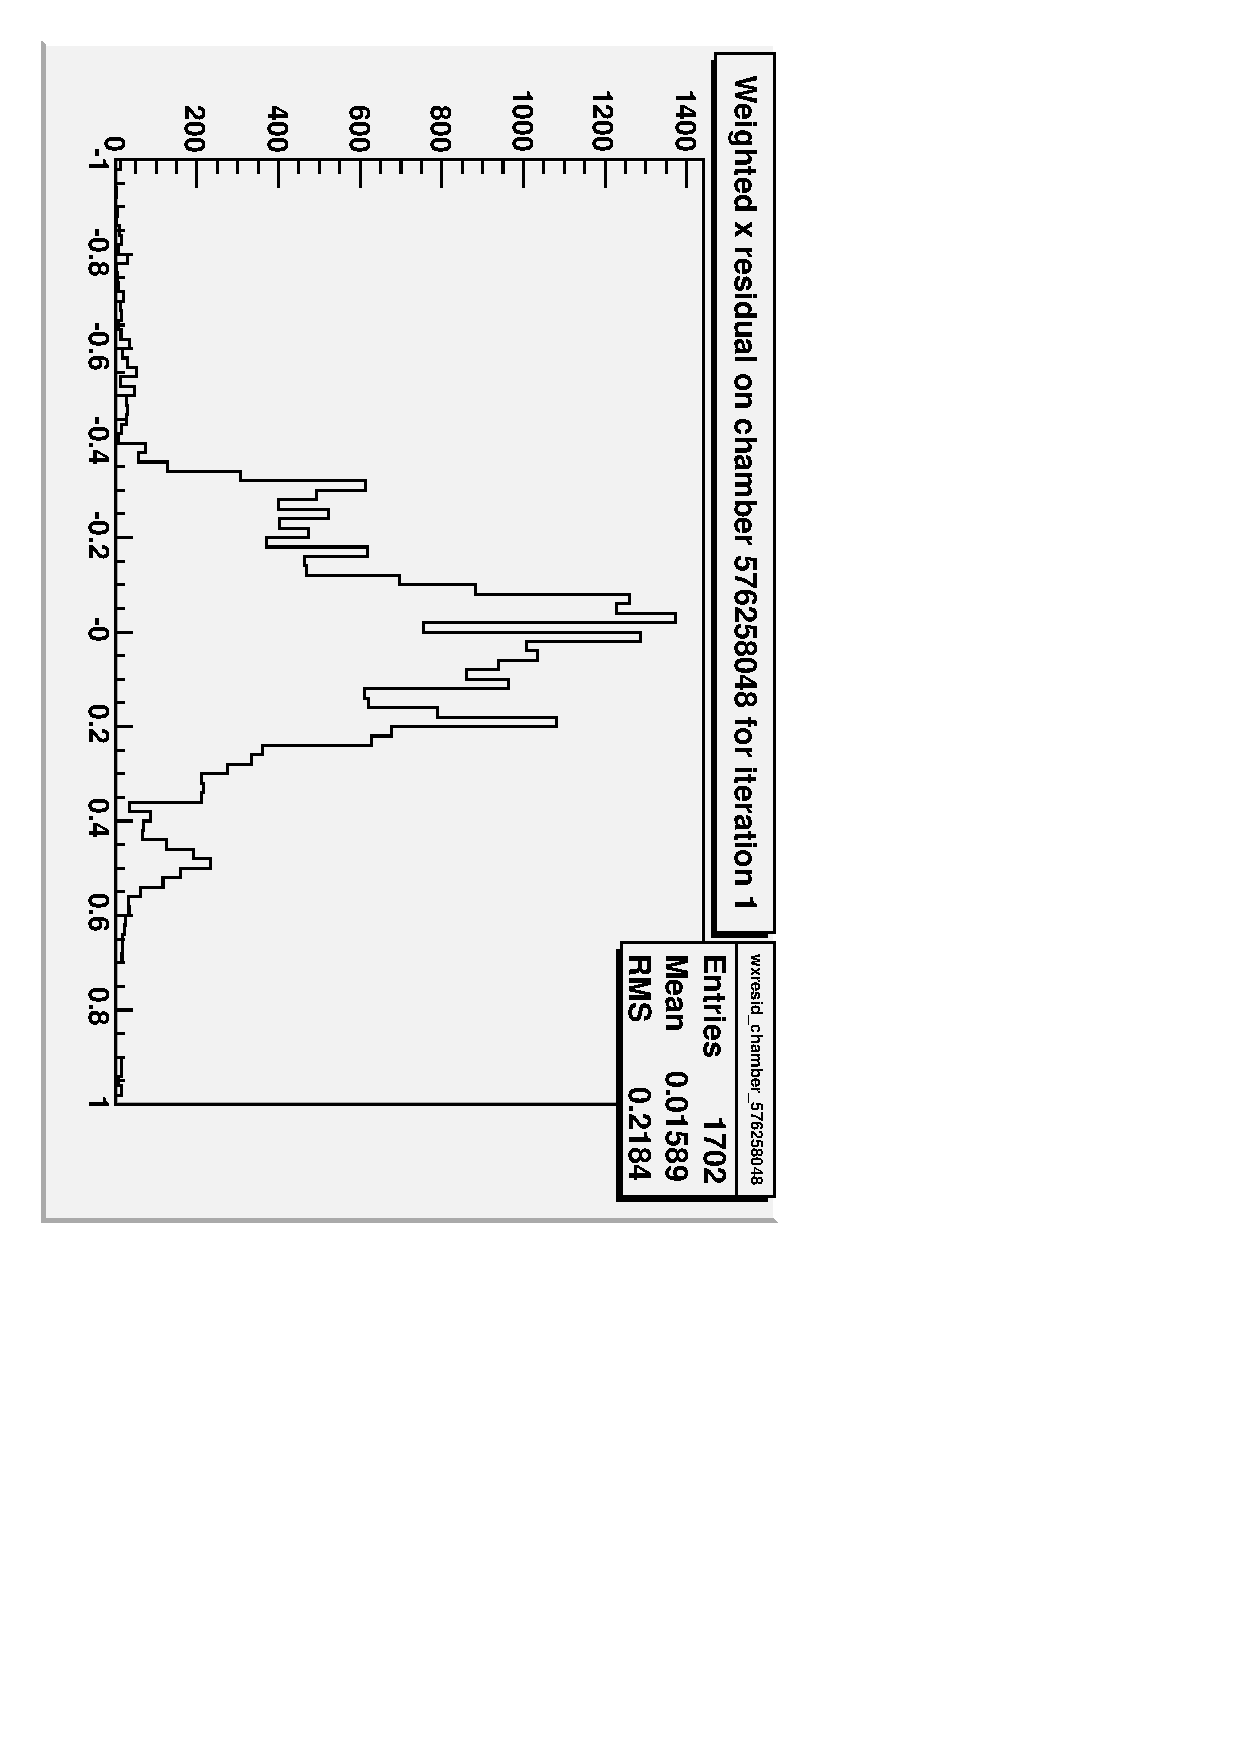
\includegraphics[height=0.7\linewidth, angle=90]{typical2_short_deweight_outin.pdf}
%% \end{center}

%% \vfill Internal structure.  Muon alignment short-term scenario does
%% not include internal (layer) misalignment.  Does calibration?
%% \end{frame}

\begin{frame}
\frametitle{Is this the right amount of misalignment?}

\begin{center}
\begin{tabular}{p{0.5\linewidth} p{0.5\linewidth}}
\begin{minipage}{\linewidth}
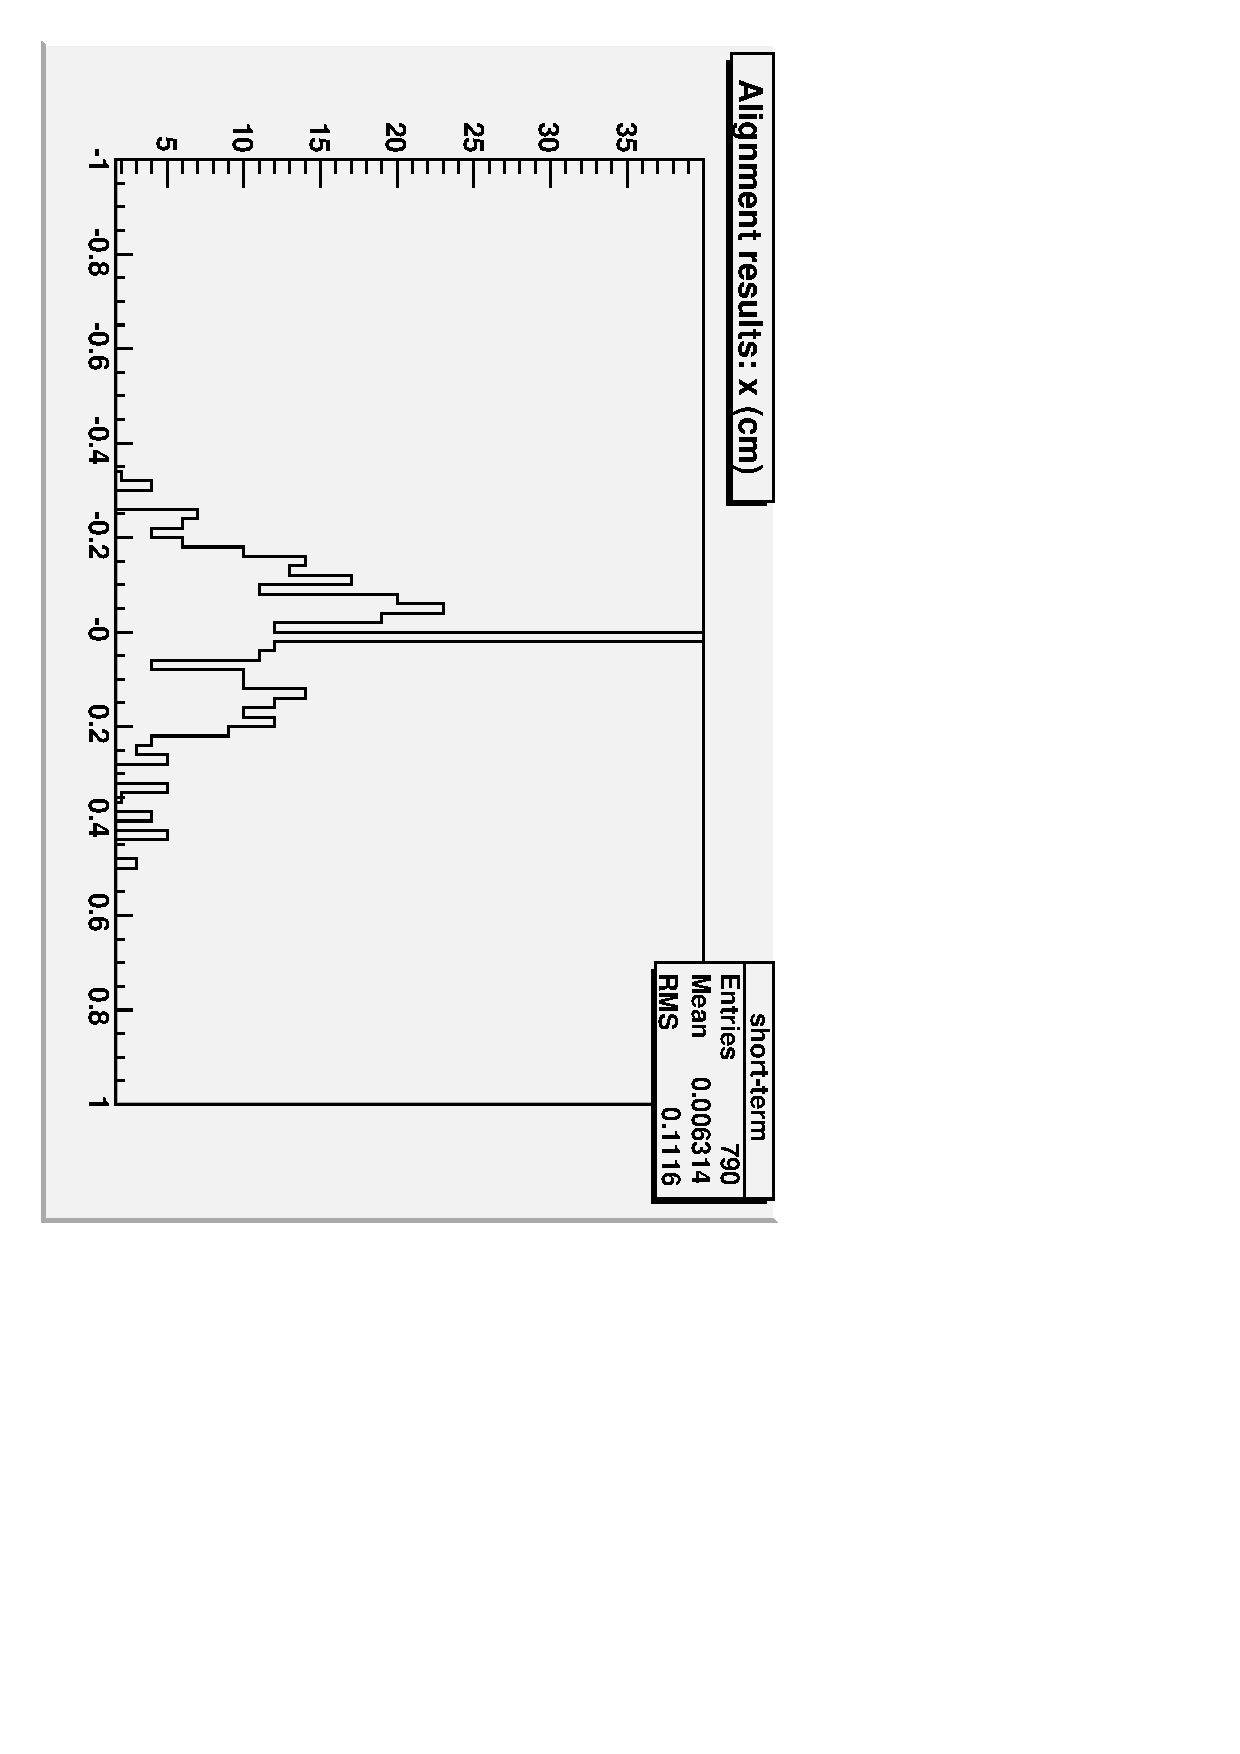
\includegraphics[height=\linewidth, angle=90]{alignment_results_x.pdf}
\end{minipage} &
\begin{minipage}{\linewidth}
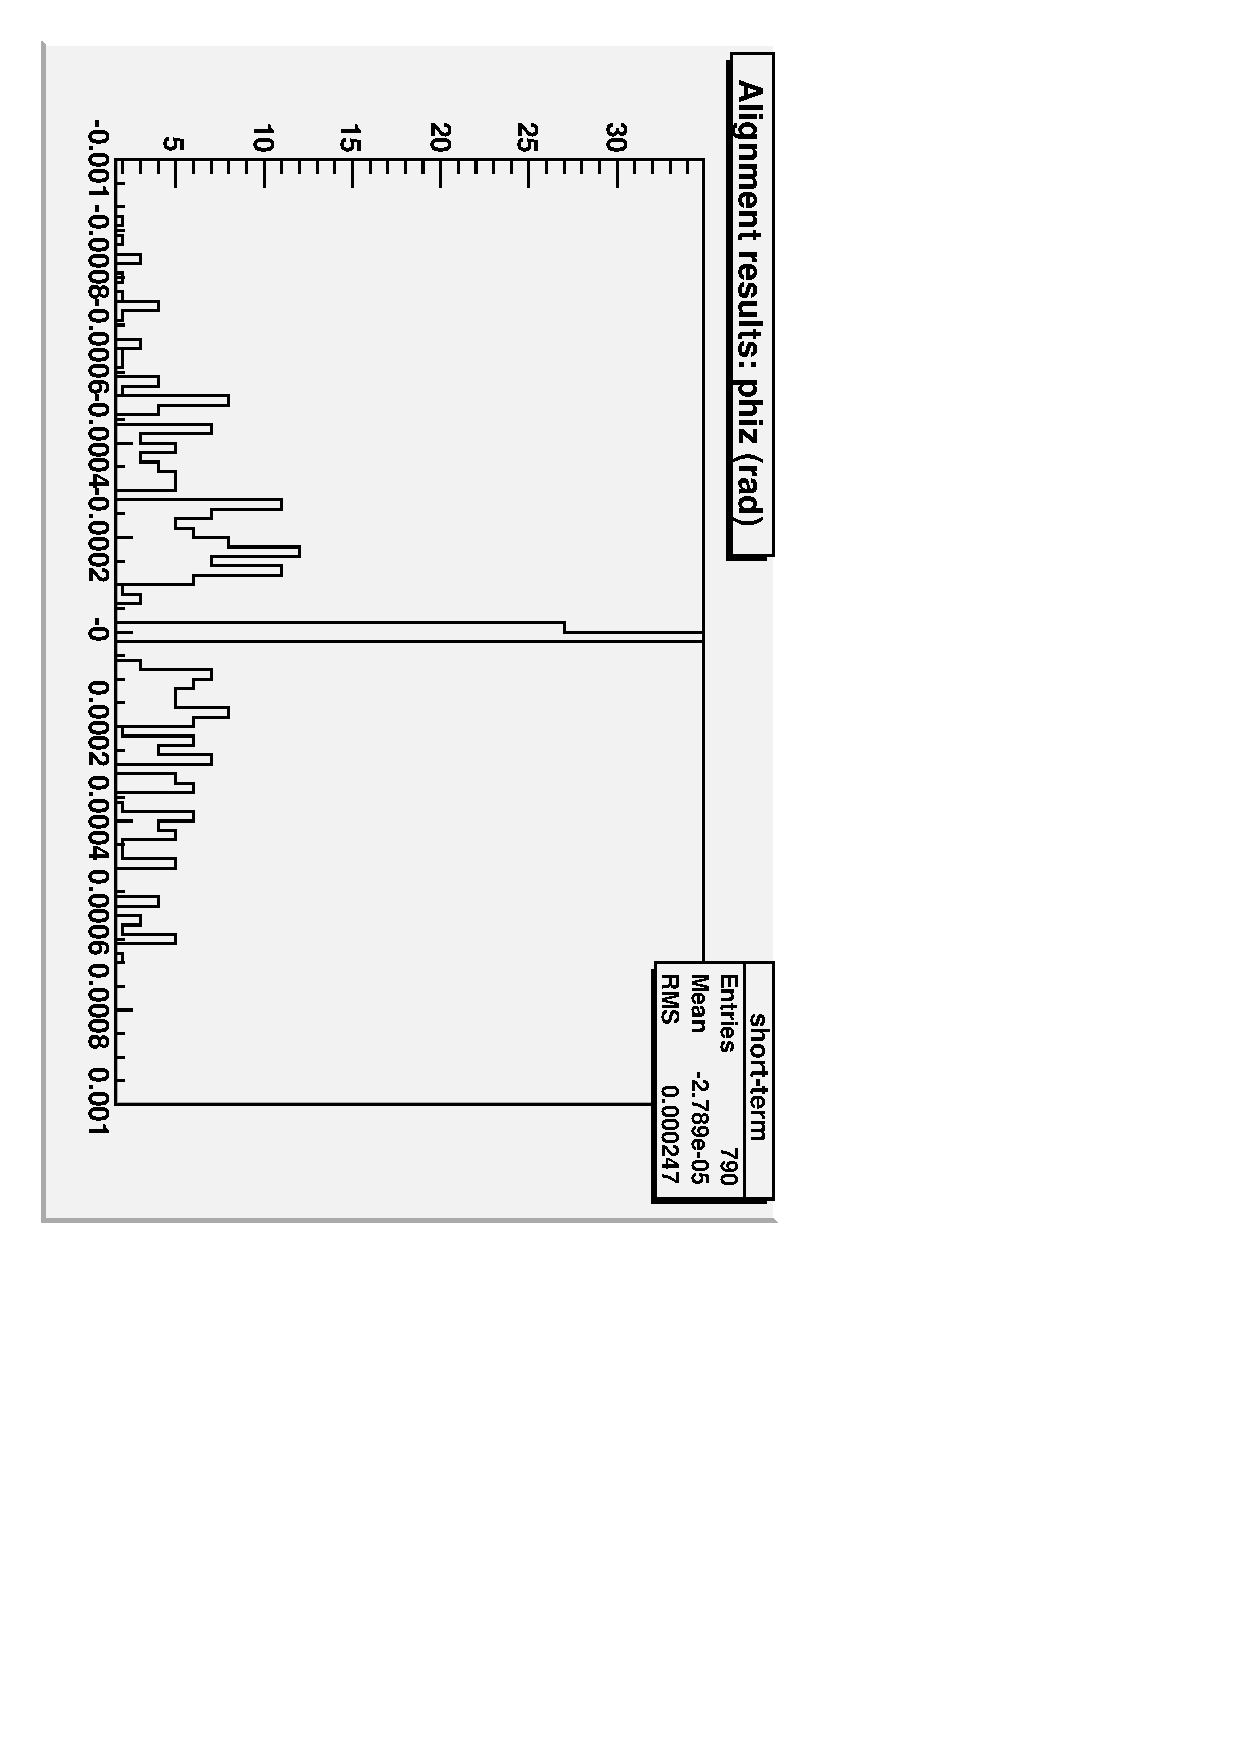
\includegraphics[height=\linewidth, angle=90]{alignment_results_phiz.pdf}
\end{minipage} \\
 & \\
\begin{minipage}{\linewidth}
\textcolor{blue}{Yes:} $x$ misalignment dominated by wheel/disk, 0.2--0.25 cm
\end{minipage} &
\begin{minipage}{\linewidth}
\textcolor{blue}{Yes:} $\phi_z$ both wheel/disk and chamber, 0.25 mrad
\end{minipage}
\end{tabular}
\end{center}

\vfill \vfill (Majority of chambers did not align because they didn't have the
minimum number of required hits)

\vfill \mbox{ }
\end{frame}

\begin{frame}
\frametitle{Status}

\begin{itemize}\setlength{\itemsep}{0.5 cm}
\item Systematics studies will wait for official AlCaReco production (``this week'')

\item Meanwhile: MTCC alignment--- track fits look {\it too} good.  \\
I should

\begin{itemize}\setlength{\itemsep}{0.25 cm}
  \item look at layer-by-layer residuals

  \item try fitting tracks to some chambers and projecting them to
  others

  \vspace{0.25 cm}
  I think this will be a good way of factorizing the problem
  and understanding the track-fitting algorithm better (and I know how
  to do it)

  \item Alexey K.: are you available to work on this?  Can we discuss
  this to share what I've learned?

\end{itemize}
\end{itemize}

\label{numpages}
\end{frame}

\end{document}
